\documentclass{article}
\usepackage{standalone}
\usepackage{import}
\usepackage{xcolor}

\usepackage{subfigure}

%\usepackage{standalone}
\usepackage{fancyhdr}


\usepackage{import}
\usepackage{caption}
\usepackage{amsfonts, amsmath, amsthm}
\usepackage{makecell}
\usepackage{lastpage}
\usepackage{moresize}



\hyphenpenalty=10000


\usepackage[utf8x]{inputenc}
\usepackage[T1]{fontenc}
\usepackage[english]{babel}
\usepackage{graphicx}
%\usepackage[languagenames,fixlanguage,english]{babelbib}
\usepackage[pdftex]{hyperref}
%\usepackage{txfonts}
%\usepackage{subcaption}
\usepackage[a4paper,top=3cm,bottom=2cm,left=3.5cm,right=3.5cm,marginparwidth=1.75cm]{geometry}
\usepackage{algorithm2e}
\usepackage{pdflscape}

\usepackage[e, gameslogo]{Template/gameshf}






\usepackage{tikz}
\usepackage{pgfplots}
\usepackage{circuitikz}
\usepackage{tabularx}
\usepackage{rotating}
\usepackage{caption} 
\captionsetup[table]{skip=10pt}

\usetikzlibrary{calc,positioning,shapes,decorations.pathreplacing}

\tikzset{
	short/.style={draw,rectangle,text height=3pt,text depth=13pt,
		text width=7pt,align=center,fill=gray!30},
	long/.style={short,text width=1.5cm},
	verylong/.style={short,text width=4.5cm}
}


%% User defined
\newcommand{\N}{\mathbb{N}}
\newcommand{\Z}{\mathbb{Z}}
\newcommand{\Q}{\mathbb{Q}}
\newcommand{\R}{\mathbb{R}}
\newcommand{\C}{\mathbb{C}}
\newcommand{\funcA}{\mathfrak{a}}
\newcommand{\funcB}{\mathfrak{b}}
\newcommand{\funcC}{\mathcal{C}}
\newcommand{\funcU}{\mathcal{U}}
\newcommand{\funcV}{\mathcal{V}}
\newcommand{\funcW}{\mathcal{W}}
\newcommand{\simgrad}{\sym\nabla}
\newcommand{\heps}{{h,\varepsilon}}
\newcommand{\epsh}{{\varepsilon(h)}}
\newcommand{\eps}{{\varepsilon}}
\newcommand{\twoscale}{{\,\overset{2}{\rightharpoonup}\,}}
\newcommand{\drtwoscale}{{\,\overset{dr-2}{\rightharpoonup}\,}}
\DeclareMathOperator{\sym}{sym}
\DeclareMathOperator{\dvg}{div}

%\newtheorem{exmp}{Example}[section]
%\newtheorem{note}{Note}
%\newtheorem{theorem}{Theorem}[section]
%\newtheorem{proposition}[theorem]{Proposition}
%\newtheorem{corollary}{Corollary}
%\newtheorem{definition}[theorem]{Definition}
%\newtheorem{lemma}{Lemma}[theorem]

\headheight 40pt              %% put this outside
\headsep 10pt                 %% put this outside


\graphicspath{{./Images/Crane/}{./Images/Electronics/}{./Images/}}

% Source: 
%https://tex.stackexchange.com/questions/117990/unicode-math-breaks-declaremathoperator
\AtBeginDocument{
	\let\div\relax
	\DeclareMathOperator{\div}{div}
}

\usepackage{enumitem}
\setlist[description]{style=unboxed}

%opening
\title{STEM games 2019}
\author{Mentori}

\title{STEM Games Engineering Arena}
\date{}

\begin{document}
	%\maketitle
	
	\thispagestyle{empty}
	\newpage
	\thispagestyle{empty}
	\vspace*{0cm}
	\begin{center}
		
		\textbf{\Huge{STEM Games 2019}}\\
		\vspace*{2.4cm}
		
\includegraphics[width=0.4\textwidth]{logos/engineering} \\
		\vspace*{2.4cm}
		% TODO naslov
		\huge{UNDERWATER HABITATS}
		
		\medskip
		
		\normalsize{a problem by}
		
		\medskip
		
		Dominik Barbarić \\
		Karla Draženović \\
		Nenad Ferdelji \\
		Luka Mandić \\
		Ante Orešković \\
		Ivan Pavić \\
		Vedran Slapničar \\
		Danijel Zadravec \\
		Marko Švec 
		
		\vspace{6cm}
		
		
		% TODO Neki mini tekst?
		\normalsize{}
	\end{center}
	
	\newpage
		
	\section{Introduction}
	
	The choice of propulsion system type is one of the most important parts in submarine’s design process since it determines the ability of fulfilling its purpose. Submarines that perform underwater research activities require endurance and certain flexibility in different littoral conditions. For example, conventional motor propulsion systems, such as diesel electric, when operational, require fresh air intake for driving electrical generator. In this way, a period while a submarine can remain submerged is limited by the power and endurance of the battery system and counts in hours or few days at most. Therefore, when it comes to endurance such systems might not be an optimal choice. Technology that overcomes this drawback is a nuclear power system which offers better endurance (even few months) and speed of the submarines but there are number of disadvantages (very expensive, operational limitations in shallow littoral waters etc.) that make them unsuitable for underwater research activities. The most suitable seems to be so called Air Independent Propulsion systems (AIP systems) which are marine propulsion technologies that allows non-nuclear submarine to operate without access to atmospheric oxygen. 
	
	One of the most interesting is definitely French AIP technology so called 
	MESMA (Module d'Energie Sous-Marine Autonome). This is the AIP system that 
	uses closed-turbine cycle for powering electrical generator and the heat 
	for steam generation is provided by liquid bioethanol combustion in pure 
	oxygen. Combustion of pure bioethanol makes this system ecologically much 
	more acceptable than other systems that use conventional fuels. In this 
	way, virtually silent MESMA exploits all advantages of AIP systems for 
	maintenance of underwater habitats and performing underwater research or 
	training activities.
	
	
	The assignment can be divided into two steps: 
	
	\begin{enumerate}
		\item Design and dimension main components of the propulsion system,
		\item Define operational characteristics of some components.
	\end{enumerate}

	After the first step you will be given a full model of propulsion system with the components you selected which will help you define operational characteristics of some components.
	Detailed description of the system components is given in the next section.
	
	Engineers, good luck!
		
	\newpage
	\section{Power generation system description}
	
	
	\subsection{The submarine}
	
	Today's assignment is to design a MESMA power generation system for 
	submarine propulsion for a given submarine hull which consists of outer and 
	inner shell, showed on Figure \ref{fig:side_view}. Inside inner shell 
	there is a reserved space of fixed volume consisting of five compartments;
	power system comparment (compartment 5), bioethanol tank (compartment 4), 
	liquid oxygen tank (compartment 3), cargo storage (compartment 2), and crew 
	deck (compartment 1).
	
	
	\begin{figure}[h!]
		\centering
		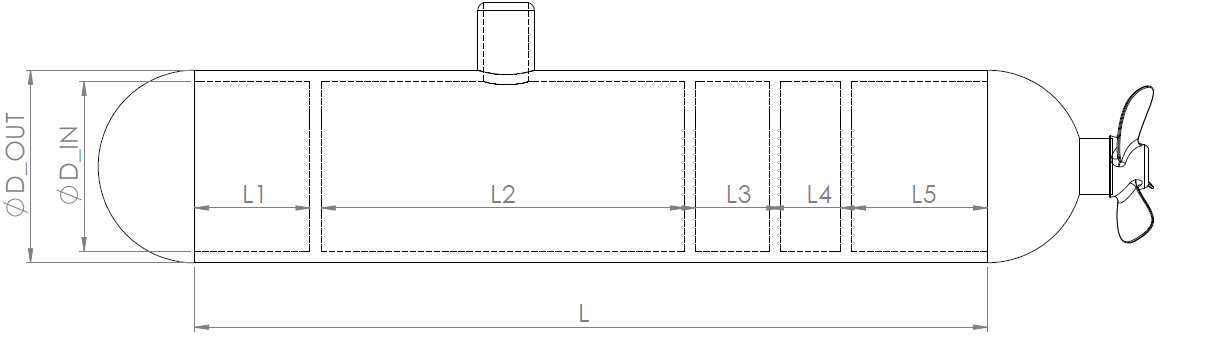
\includegraphics[width=\textwidth]{submarine_side_view.png}
		\caption{Submarine dimensions}
		\label{fig:side_view}
	\end{figure}
	
	The following dimensions are given:
	\begin{itemize}
		\item $L = 18 \,\textrm{m}$
		\item $D_{OUT} = 1.7 \,\textrm{m}$
		\item $D_{IN} = 1.5 \,\textrm{m}$
		\item $L_1 = 2 \,\textrm{m}$
	\end{itemize}
	
	$D_{IN}$  is used for the tank volume calculation.

	Also, dimension $L_5$ is found as
	\begin{equation}
		L_5 = (18 \cdot P_\textrm{turb} + 2500)/1000 \,\left[\textrm{m}\right]
	\end{equation}
	where the power $P_\textrm{turb}$ is taken in kW. Dimensions $L_2$ and 
	$L_3$ depend on the chosen amount of fuel and oxygen.
	
	Team's solutions will be ranked in the following categories:
	\begin{itemize}
		\item Maximum speed
		\item Maximum range
		\item Maximum depth
		\item Available cargo volume
	\end{itemize}
    Each category can win you up to 25\% of points available for this task. The 
    team that achieved the highest score in each category will be awarded the 
    maximum number of points. The other teams' points will be scaled 
    accordingly.

	
	
	\subsection{Power system}
	
	Power generation system schematics are shown on figure \ref{fig:pwr_scheme}.
	
	\begin{figure}[h!]
		\centering
		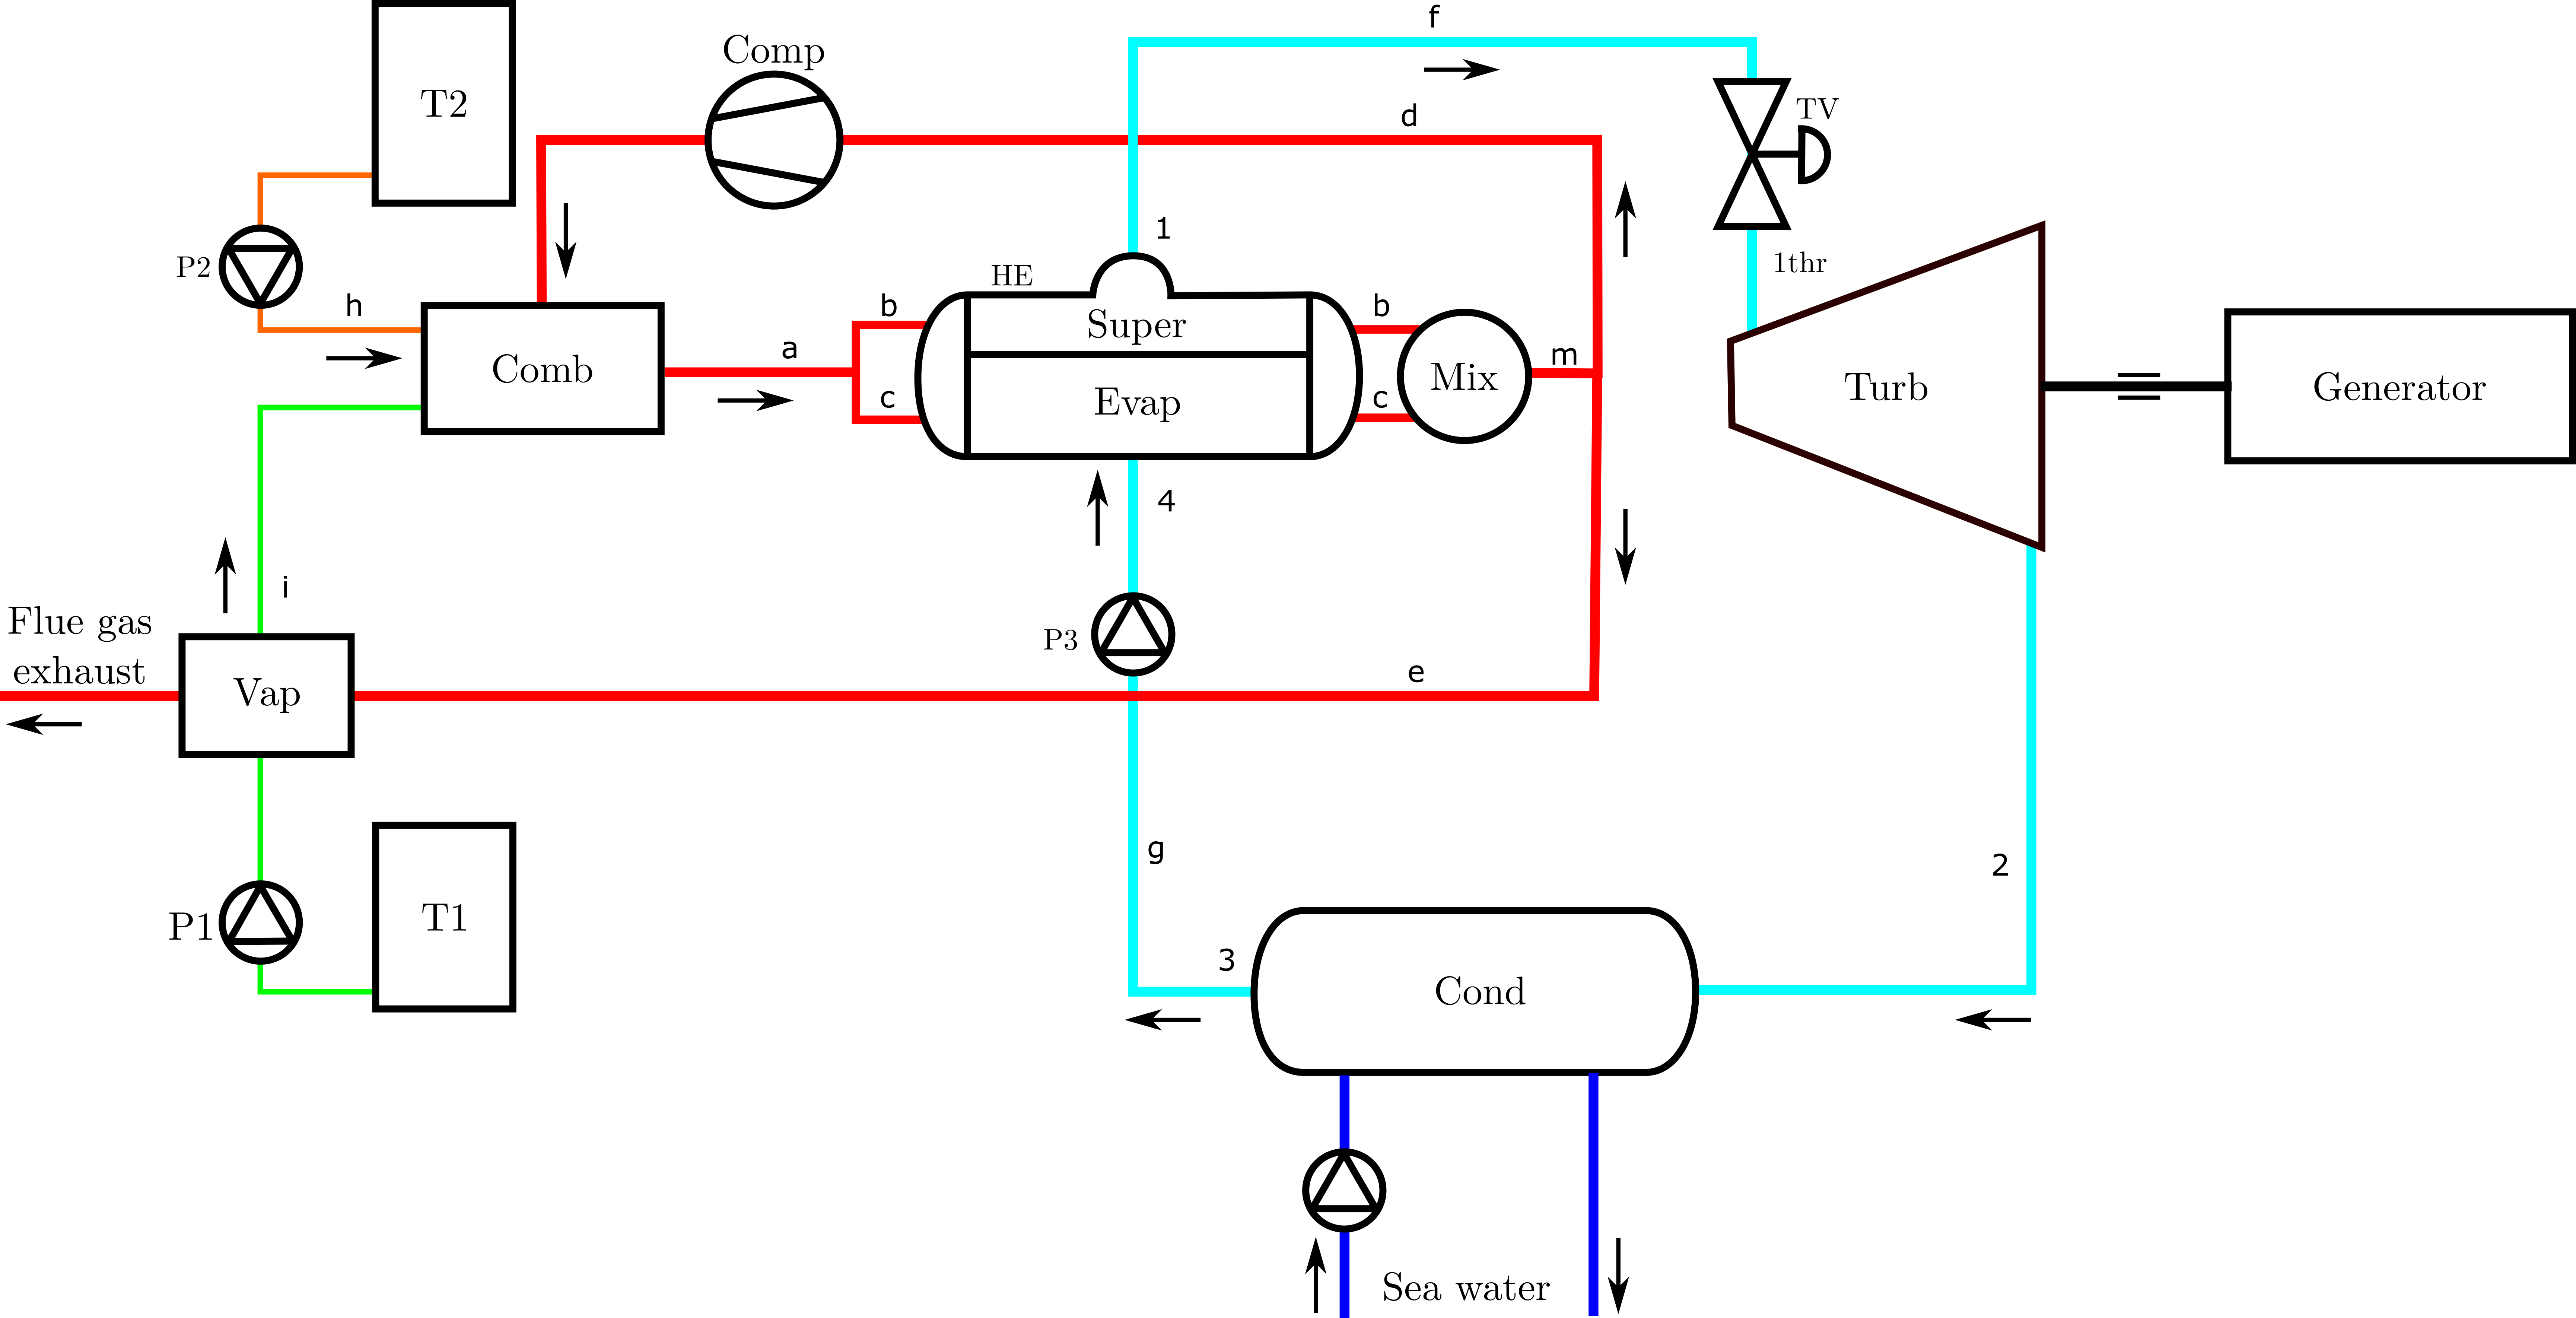
\includegraphics[width=\textwidth]{terma.png}
		\caption{Power generation system}
		\label{fig:pwr_scheme}
	\end{figure}
	
	Submarine power generation system consists of two main circuits; \\
	flue gas\footnote{combustion exhaust gas} circuit (red) and steam 
	circuit (cyan). 
	Steam circuit is used for steam production which expands in turbine "Turb" 
	providing necessary power for the "Generator" used for charging the 
	batteries for submarine propulsion. The flue gas circuit is used to provide 
	necessary heat flow for evaporating and superheating the steam for the 
	turbine. Flue gas is generated in the combustion chamber "Comb" in which 
	energy is released by ethanol combustion in pure oxygen.
	
	Liquefied oxygen and ethanol fuel are stored in separate tanks "T1" and 
	"T2", respectively. While pump P2 delivers fuel stream "h" to combustion 
	chamber "Comb", cryogenic pump P1 delivers liquefied oxygen stream "i" to 
	oxygen vaporizer "Vap" where it vaporizes and enters combustion chamber 
	"Comb" in stoichiometric ratio at which fuel combustion is, by assumption, 
	complete without any excess oxygen. Flue gas temperature at the outlet from 
	the combustion chamber (stream "a") is controlled by return stream of 
	cooled flue gas "d" by compressor "Comp" and\\
	 should never exceed maximum allowed flue gas temperature %ϑ_(fg,max).
	
	Flue gas stream "a", which exits combustion chamber "Comb" enters heat 
	exchanger "HE" used for water evaporation and steam superheating. 
	Therefore, heat exchanger "HE" comprises two sections; an evaporation 
	section "Evap" and superheating section "Super". Total 
	flue gas mass flow which enters heat exchanger "HE" is divided into two 
	flue gas streams "b" and "c". Stream "c" flows through evaporation ("Evap") 
	section and stream "b" flows through superheating ("Super") section in 
	parallel configuration. On heat exchanger exit, two flue gas parallel 
	streams "b" and "c" are adiabatically mixed in mixing chamber "Mix" forming 
	flue gas stream "m".Part of stream "m" is returned by compressor "Comp" to 
	combustion chamber "Comb" as stream "d" to prevent overheating (maximum 
	allowed flue gas temperature), while the rest (stream "e") is used for 
	oxygen evaporation in heat exchanger "Vap" and evacuated outside submarine.
	  
	Heat exchanger "HE" is a pool boiling type apparatus which means that liquid water in the evaporating section is at rest and is evaporated by the flue gas that passes through a tube bundle in the evaporating section. The exact amount of steam that is evaporated in evaporation section "Evap" (which corresponds to the steam mass flow of stream "g") is then superheated in superheating section "Super" of heat exchanger "HE" producing the superheated steam "f". Superheated steam (stream "f") passes through throttling valve "TV" and enters the steam turbine "Turb" where mechanical power is produced by steam adiabatic expansion to condensation pressure p2. After the expansion, low pressure steam condenses in sea water cooled condenser "Cond" and is returned to high pressure evaporator "Evap" by condensate pump "P3". 
	
	
	Following sections provide a detailed description of every part of power 
	generation system that should be modeled.
	
	
	It is very important that system states are in allowed limits. 
	
	\begin{itemize}
		\item Maximum temperature at combustion chamber “Comb“ exit 
		(850$^\circ$)
		\item Maximum steam temperature at turbine “Turb” inlet (Excell table 1)
		\item Minimum vapor fraction on turbine “Turb” outlet (0.9)
		\item Evaporator “Evap” erosion (given by the equation 
		\ref{eq:flue_gas_density})
		\item Superheater “Super” erosion (given by the equation 
		\ref{eq:flue_gas_density})
		\item System malfunction due to insufficient generated power (given by 
		the equation \ref{eq:minpower})
	\end{itemize}

	Each failed test will cause 40\% point reduction in the given test category.
	
	\subsection{Turbine}
	
	A Steam Turbine is a mechanical device in which thermal energy is extracted from pressurized steam by its adiabatic expansion and is transformed to mechanical work.  Therefore, for a given mass flow rate of steam qm, power $P$ generated by steam turbine is defined:
	
	\begin{equation}\label{eq:power}
		P = q_m(h_1 - h_2),
	\end{equation}
	
	\noindent
	where 
	
	\begin{itemize}
		\item $q_m$ is steam mass flow rate, 
		\item $h_1$ is steam specific enthalpy at turbine inlet,
		\item $h_2$ is steam specific enthalpy at turbine outlet.
	\end{itemize}

	Turbine steam swallowing capacity mass flow rate $q_m$ at given pressures and inlet temperature can be expressed by Stodola’s Ellipse equation:
	
	\begin{equation}\label{eq:stodola}
		q_m = \frac{K}{\sqrt{T}}(p_1^2 - p_2^2)^\frac{1}{2},
	\end{equation}
	
	\noindent
	where:
	
	\begin{itemize}
		\item $K$ is Stodola’s coefficient $\left[\frac{\sqrt{\textrm{K}}\cdot 
		\textrm{kg}}{\textrm{s} \cdot \textrm{\textrm{bar}}}\right]$, 
		\item $p_1$ is turbine inlet pressure $\left[\textrm{bar}\right]$,
		\item $p_2$ is turbine outlet pressure $\left[\textrm{bar}\right]$,
		\item $T$ is turbine inlet absolute temperature 
		$\left[\textrm{K}\right]$.
	\end{itemize}
	
	\subsubsection*{Steam turbine isentropic efficiency}
	
	Turbine isentropic efficiency $\eta$ is defined as the ratio between enthalpy drop at actual turbine expansion and enthalpy drop at isentropic expansion between inlet and outlet turbine pressure $p_1$ and $p_2$.
	
	\begin{equation}\label{eq:eta}
		\eta = \frac{h_1-h_2}{h_1 - h_{2s}}.
	\end{equation}
	
	Steam turbine isentropic efficiency depends upon mean steam volume flow 
	rate $q_v$ according to the following equation:
	
	\begin{equation}\label{eq:eta2}
		\eta = aq_v^2 + bq_v + c,
	\end{equation}
	
	\noindent
	where $q_v$ is geometric mean of volume flow rates at turbine inlet ($q_{v,in}$) and at outlet in case of isentropic expansion ($q_{v,out,s}$). 
	
	\begin{equation}\label{eq:q_v}
		q_v = \sqrt{q_{v,in} \cdot q_{v,out,s}},
	\end{equation}
	
	Turbine efficiency is highest at its nominal design point for which 
	pressures ($p_1$, $p_2$) and inlet temperature T1 are given in Excel Table 
	1, while nominal flow rate is defined by Stodola’s Ellipse equation 
	\ref{eq:stodola}. Turbine can operate at other conditions (off design 
	turbine performance with lower, i.e. higher mass flow rates than the 
	nominal) with the cost of reduced efficiency, provided that these 
	conditions are not outside permitted values.
	
	\subsubsection*{Off design turbine performance}
	
	\subsubsection*{Lower mass flow rate}
	
	Steam throttling is a common way for reduction of power produced by steam 
	turbine. By reducing fuel pump "P2" and oxygen pump "P1" speed accordingly 
	when power demand is lowered, fuel consumption and evaporated steam mass 
	flow rate are decreased. In conjunction with steam flow rate decrease, 
	throttling valve "TV" orifice is constricted to reduce turbine inlet 
	pressure $p_{1,thr}$ to a value which satisfies Stodola’s Ellipse law 
	\ref{eq:stodola} for given decreased mass flow rate $q_m$. In a throttling 
	process, superheated steam which exits heat exchanger "HE" is throttled to 
	lower pressure $p_{1,thr}$, while steam enthalpy is conserved.
	
	\begin{equation}\label{eq:ent_preserve1}
		h_{1,thr} = h_1,
	\end{equation}
	\begin{equation}\label{eq:ent_preserve2}
	p_{1,thr} = p_1,
	\end{equation}
	\begin{equation}\label{eq:ent_preserve3}
	T_{1,thr} = T(p_{1,thr},h_1) < T_1.
	\end{equation}
	
	Side effect of throttling is a temperature reduction which corresponds to the state of conserved enthalpy $h_1$ at throttled pressure $p_{1,thr}$. Pressure and temperature are both part of a Stodola’s Ellipse law \ref{eq:stodola} which means they need to simultaneously satisfy Stodola’s Ellipse law  \ref{eq:stodola}  and enthalpy conservation of a throttling process from state "1".
	
	By throttling, turbine inlet pressure and inlet temperature are reduced which decreases available isentropic power of turbine. Turbine efficiency described by equation \ref{eq:eta2} is also decreased at partial turbine load.
	
	\subsubsection*{Higher mass flow rate}
	
	In case that power demand is increased, turbine can be overloaded by steam mass flow $q_m$ greater than nominal. This is achieved by fuel pump "P2" and oxygen pump "P1" speed increase which causes increased fuel consumption and evaporated steam mass flow. When turbine is overloaded, steam flow bypasses few initial turbine stages which enables increased steam consumption, although with reduced turbine efficiency described by equation (4). To accurately model this effect is out of scope of this assignment. Therefore, it is assumed in overload working mode that turbine inlet values of pressure and temperature remain nominal, i.e. there is no change at throttling valve due to increased steam mass flow rate $q_m$. The only effect of increased $q_m$ is turbine efficiency reduction as described by equation \ref{eq:eta2}.
	
	Restrictions of steam turbine operational parameters are following:
	
	\begin{itemize}
		\item Steam temperature at turbine inlet should not exceed temperature $\vartheta_{turb,max}$,
		\item Define operational characteristics of some components.
	\end{itemize}
	
	\noindent
	\textcolor{red}{Turbine design parameters are given in Excel Table 1.}

	\subsubsection*{Minimum required turbine power}
	
	The minimum power which the turbine has to provide for the submarine for it 
	to remain operational is defined by
	\begin{equation}\label{eq:minpower}
	P_\textrm{min} = 2 + 0.05 \cdot P_\textrm{nom} \ \left[\textrm{kW}\right]
	\end{equation}
	where $P_\textrm{nom}$ is the nominal turbine power, given in Excel Table 1 
	in kW.

	If the power generated by the turbine falls below the value of 
	$P_\textrm{min}$, the submarine will fatally malfunction.

	Submarine velocity is calculated based on the power remaining for 
	propulsions, as
	\begin{equation}
	v_\textrm{sub} = 2.0135 \cdot P_\textrm{prop}^{0.3518} \ 
	\left[\textrm{kn}\right]
	\end{equation}
	where $P_\textrm{prop}$ is taken in kW, and it is equal to
	\begin{equation}
	P_\textrm{prop} = P_\textrm{turb} - P_\textrm{min}
	\end{equation}
	
	\subsection{Heat exchangers}
	
	Heat exchanger is a device whose purpose is to transfer heat from warmer 
	fluid stream to colder stream. There are three heat exchangers in the power 
	generation system: heat exchanger "HE" which is divided to superheating and 
	evaporative section, condenser "Cond" and oxygen vaporizer "Vap". Condenser 
	"Cond" and vaporizer "Vap", whose performance will not be evaluated in this 
	task are assumed to be regulated accordingly in each time step with the 
	current need of the power generation system. 
	
	\subsubsection*{Heat exchanger "HE"}
	
	Heat exchanger "HE" is used for steam evaporation and superheating in two corresponding sections by hot flue gas from combustion chamber ("b" and "c" stream). It is shell and tube type with flue gas passing through tubes in each section. 
	
	Heat flow exchanged in each of two heat exchanger sections is described as:
	
	\begin{equation}\label{eq:heat_flow}
		\Phi = A \cdot k \cdot LMTD,
	\end{equation}
	
	where:
	
	\noindent
	$LMTD$ is logarithmic mean temperature difference, 
	$k$ is overall heat transfer coefficient,
	$A$ is total heat exchange area of the section. 
	Assume superheating section of heat exchanger is counter-flow.
	
	In addition to LMTD method, rate of heat transfer can be determined using NTU method. For counter-flow heat exchanger effectiveness is calculated as:
	
	\begin{equation}\label{eq:heat_exchanger_eff}
		\pi_1 = \frac{1 - exp((1-\pi_3)\pi_2)}{1-\pi_3exp(-(1-\pi_3)\pi_2)},
	\end{equation}
	
	Dimensionless parameters $\pi_1$,$\pi_2$,$\pi_3$ are defined as follows:
	
	\begin{equation}\label{eq:pi_params}
		\pi_1 = \frac{\theta'_1 - \theta''_1}{\theta'_1 - \theta'_2},
	\end{equation}
	
	\begin{equation}\label{eq:pi_params2}
		\pi_2 = \frac{kA}{C_1},
	\end{equation}
	
	\begin{equation}\label{eq:pi_params3}
		\pi_3 = \frac{C_1}{C_2},
	\end{equation}
	
	\noindent
	where $C$ is stream heat capacity.
	
	Index 1 corresponds to stream with lower heat capacity, index 2 to stream with higher heat capacity, superscript $'$ to stream inlet state in heat exchanger and $''$ to outlet state.
	
	Flue gas, which is divided into two streams "b" and "c" enters evaporation "Evap" and superheating "Super" section at equal temperature and flows through tubes in one pass. Flue gas mass flow through evaporative and superheating section of heat exchanger is defined as:
	
	\begin{equation}\label{eq:flue_gas_flow1}
		q_{m,fg,evap} = evap_{fr} \cdot q_{m,fg},
	\end{equation}
	
	\begin{equation}\label{eq:flue_gas_flow2}
		q_{m,fg,super} = (1-evap_{fr}) \cdot q_{m,fg},
	\end{equation}
	
	\noindent
	Where:
	$evap_{fr}$ is flue gas fraction of stream "c" to total flue gas stream "a"  total flue gas mas flow and is assumed constant throughout system operation. Its value can be selected between 0 and 1.
	$q_{m,fg}$ is total flue gas mass flow rate (stream "a") .
	$q_{m,fg,evap}$ is evaporation section mass flow rate (stream "b")
	$q_{m,fg,super}$ is superheating section mass flow rate (stream "c")
	Heat transfer coefficient on tube side can be calculated by using following simplified convection models.
	
	\noindent
	If the flow is transient or turbulent ($2300 < Re < 5e6$) , mean Nusselt number is defined as:
	
	\begin{equation}\label{eq:nusselt}
		Nu = \frac{f/8 \cdot (Re - 1000) \cdot Pr}{1+12.7\sqrt{f/8} \cdot (Pr^{2/3}-1)},
	\end{equation}
	
	\noindent
	where $f$ is the friction factor, defined as
	
	\begin{equation}\label{eq:fric_factor}
		f = \frac{1}{(1.82\log_{10}Re - 1.64)^2}.
	\end{equation}
	
	\noindent
	If the flow is laminar ($Re<2300$), mean Nusselt number is defined as:
	
	\begin{equation}\label{eq:nusselt2}
		Nu = 1.86 \left(Pe \frac{d}{L}\right)^{1/3}.
	\end{equation}
	
	\noindent
	In above equations non-dimensional numbers are
	
	\begin{itemize}
		\item $Nu = \frac{\alpha d}{\lambda}$ Nusselt number
		\item $Re = \frac{\rho w d}{\mu}$ Reynolds number
		\item $Pr = \frac{\mu c_p}{\lambda}$ Prandtl number
		\item $Pe = Re Pr$ Peclet number
	\end{itemize}

	\noindent
	Nusselt, Prandtl and Reynolds numbers and flue gas velocity are calculated using mean flue gas temperature properties between pipe inlet and outlet. All physical properties except density are assumed independent of pressure and its values for pure gases are given in appendix. Flue gas physical properties are calculated as molar average of gases which form flue gas. Density is calculated using ideal gas equation of state.
	
	\noindent
	Evaporation occurs on shell side of evaporative section of heat exchanger. Evaporative heat transfer coefficient on shell side is assumed constant and its value is $\alpha_{ev}=3500 \frac{W}{m^2 K}$. In superheater section of exchanger, heat transfer coefficient on shell side is also assumed constant and its value is $\alpha_{super}=70 \frac{W}{m^2 K}$.
	
	Evaporated steam mass flow $q_m$ is determined by heat flow $\Phi_e$ exchanged in evaporative part "Evap" of heat exchanger "HE":
	
	\begin{equation}\label{eq:evap_steam_mass}
		\Phi_e = q_m(h'' -h_4),
	\end{equation}
	
	where $h''$ is saturated (dry) steam specific enthalpy, and $h_4$ is 
	enthalpy of subcooled liquid at condensate pump outlet. 
	The same amount of heat flow is received from stream "b" flue gas whose enthalpy decreases.
	
	\begin{equation}\label{eq:evap_steam_mass2}
		\Phi_e = q_{m,fg,evap} (h_{fg,comb} - h_{fg,evap,out}),
	\end{equation}
	
	\noindent
	where 
	$h_{fg,comb}$ is flue gas specific enthalpy at combustion chamber "Comb" outlet
	$h_{fg,evap,out}$ is flue gas specific enthalpy at evaporative section "Evap" outlet.
	Flue gas mean molar heat capacities are given in appendix
	It is assumed that mass flow $q_m$ in current time step flows through superheating section "Super" of "HE", turbine "Turb", condenser "Cond" and condensate pump "P3".
	
	Evaporated steam mass flow $q_m$, whose value is determined by equation 
	(13) is then superheated at constant pressure in superheater section 
	"Super" of heat exchanger "HE" by exchanged heat flow:
	
	\begin{equation}\label{eq:evap_steam_mass3}
		\Phi_s = q_m(h_1 - h''),
	\end{equation}
	
	The same amount of heat flow is received from stream "c" flue gas whose enthalpy decreases.
	
	\begin{equation}\label{eq:evap_steam_mass4}
		\Phi_s = q_{m,fg,super} (h_{fg,comb} - h_{fg,super,out}),
	\end{equation}
	
	\noindent
	where $h_{super,out}$ is flue gas specific enthalpy at superheating section "Super" exit. Both flue gas streams are adiabatically mixed at heat exchanger outlet in mixing chamber "Mix". Outlet temperature from the mixing chamber is defined by equation:
	
	\begin{equation}\label{eq:outlet_temp}
		\Theta_{fg,ret} = \frac{q_{m,fg,evap} \cdot h_{fg,evap,out} + q_{m,fg,super} \cdot h_{fg,super,out}}{q_{m,fg} \cdot c_{p,fg} (\Theta_{fg,ret})},
	\end{equation}
	
	\noindent
	where:
	
	\begin{itemize}
		\item $q_{m,fg}$ is temperature after stream "b" and "c" mixing at which part of flue gas is returned to combustion chamber
		\item $c_{p,fg} (\Theta_{fg,ret})$ is mean specific heat capacity of flue gas between temperature $\Theta_{fg,ret}$ and $0^{\circ}C$.
	\end{itemize}
	
	\noindent
	\textcolor{red}{Data for available tubes is given in Excel Table 2.}
	
	\noindent
	Value of exchanged heat at both sections depends upon stream inlet conditions, overall heat transfer coefficient k and overall heat transfer area A. Heat transfer coefficient k and area A are influenced by number of tubes in each section and its length which define tube side heat exchanger coefficient and total heat transfer area.
	
	Type and length of tubes at evaporative and superheating section are equal. Number of tubes for each section and flue gas fraction which enters each section can be selected independently.  
	
	While designing a heat exchanger, to prevent tube erosion, one must 
	consider that product of flue gas density, $\rho$, and squared velocity, 
	$w^2$, never exceed $6800$  Pa,  i.e. 
	
	\begin{equation}\label{eq:flue_gas_density}
		\rho w^2 < 6800 Pa.
	\end{equation}
	
	\subsubsection*{Condenser}
	
	\noindent
	Condenser "Cond" is a heat exchanger which is used for condensation of steam which exits turbine "Turb" at condensation pressure $p_2$. During condensation, following heat flow is released:
	
	\begin{equation}\label{eq:heat_flow_cond}
		\Phi_{cond} = q_m (h_2 - h'),
	\end{equation}
	
	\noindent
	where $h'$ is enthalpy of saturated liquid water at condensation pressure $p_2$.
	
	\noindent
	Heat flow $\Phi_{cond}$ is rejected to sea water inside condenser "Cond". 
	It can be assumed that condenser "Cond" in the system is properly designed 
	and sea water mass flow at pump "P4" is automatically adjusted to absorb 
	heat flow $\Phi_{cond}$. Therefore, sizing of condenser "Cond" and sea 
	water pump "P4" and its control is not a part of this task and is assumed 
	as ideal. Condensed water always exits condenser "Cond" at saturated liquid 
	state.
	Maximum sea water temperature at which submarine has to operate is $30^{\circ}C$, and minimal temperature difference between condensing steam and sea water for given condenser is $15^{\circ}C$. 
	
	\subsection{Combustion chamber}
	
	Combustion chamber "Comb" is enclosed space in which ethanol burns in liquid oxygen. It is assumed to be perfectly insulated. During the combustion, lower heating value of ethanol is converted into flue gas enthalpy. Combustion pressure is at least 1 bar above static pressure evaluated at submarine centerline. Pressure loss from combustion chamber "Comb" to heat exchanger "HE" can be neglected.
	
	In addition to ethanol combustion, combustion chamber "Comb" is used for mixing newly formed flue gas and cooled flow gas which passed heat exchanger "HE" and is returned to chamber "Comb" to prevent overheating. Combustion chamber inlet streams are pure oxygen stream "i" and ethanol stream "h", both at $10^{\circ}C$ and returning flue gas stream "d" at heat exchanger exit temperature  $\Theta_{fg,ret}$. The only outlet stream from the combustion chamber "Comb" is flue gas stream "a" which consists of return flue gas "d" and flue gas newly formed by combustion. 
	
	\begin{equation}\label{eq:flue_gas_stream_new}
		q_{m,fg} = q_{m,fg,new} + q_{m,fg,ret},
	\end{equation}
	
	\noindent
	Flue gas outlet temperature is defined by first law of thermodynamics applied to combustion chamber "Comb":
	
	\begin{equation}\label{eq:flue_gas_out_temp}
		\Theta_{fg,comb} = \frac{\dot{H}_{O2,in} + \dot{H}_{ethanol,in} +\dot{H}_{fg,ret} + q_{n,ethanol} \Delta H_{md}}{C_{fg}},
	\end{equation}
	
	\noindent
	where
	
	\begin{itemize}
		\item $\Delta H_{md}$ is ethanol lower heating value [kJ/kmol]
		\item $\dot{H}_{O2,in}$ is enthalpy of oxygen stream "i" at $10^\circ C$
		\item $\dot{H}_{ethanol,in}$ is enthalpy of ethanol stream "h" at $10^\circ C$
		\item $\dot{H}_{fg,ret}$ is enthalpy of returning flue gas at temperature $\Theta_{fg,ret}$
		\item $q_{n,ethanol}$ is molar flow rate of ethanol stream "h"
		\item $C_{fg}$ is mean isobaric heat capacity of flue gas stream "a" which exits combustion chamber "Comb"
	\end{itemize}

	\noindent
	Flue gas composition is the same in all system parts and is defined by complete combustion of ethanol in pure oxygen.
	
	\subsection{Fuel and oxygen pumps}
	
	Fuel pump "P2" is used to transport fuel to combustion chamber. Pump "P2" 
	has a variable frequency drive which allows precise control of fuel mass 
	flow to combustion chamber. It is assumed that combustion of delivered fuel 
	mass flow is complete and instantaneous. It is also assumed that control of 
	oxygen pump "P1" is linked to pump "P2" in a way that oxygen supply is in 
	exact stoichiometric ratio needed for complete ethanol combustion. 
	Therefore, oxygen pump "P1" dimensioning and control is not a part of this 
	assignment. 
	Fuel pump "P2" speed determines the fuel combustion rate and influences 
	evaporation and superheating of steam in heat exchanger "HE" and finally 
	power P extracted at steam turbine "Turb".
	
	\subsubsection*{Fuel pump}
	
	Fuel pump "P2" is positive displacement pump with variable speed drive. It 
	is used to transport fuel from fuel tank "T2" to combustion chamber "Comb". 
	The total differential head a pump must generate is a sum of static head 
	difference and frictional head losses: 
	
	\begin{equation}\label{eq:head_total}
		h_{tot} = h_{stat} + h_{fr}.
	\end{equation}
	
	There is no height difference between fuel tank "T2" and combustion chamber 
	"Comb". Fuel is stored at pressure of 1 atm.
	Frictional head loss is calculated based on fuel volume flow rate:
	
	\begin{equation}\label{eq:head_loss}
		h_{fr} = k_{pipe} \cdot q_{v,fuel}^2,
	\end{equation}
	
	\noindent
	where
	
	\begin{itemize}
		\item $k_{pipe}$ is pipe friction coefficient $\left[ \frac{mh^2}{l^2} \right]$
		\item $q_{v,fuel}^2$ is fuel volume flow rate
	\end{itemize}

	\noindent
	It is assumed that positive displacement pump volume flow rate depends only on pump speed and does not depend on pump head. Pump slippage is neglected. Pump volume flow rate with respect to pump speed is defined:
	
	\begin{equation}\label{eq:pump_vol_flow}
		q_v = \frac{N}{N_{max}} q_{v,max},
	\end{equation}
	
	\noindent
	where
	
	\begin{itemize}
		\item $N$ is pump speed
		\item $N_{max}$ is maximum pump speed
		\item $q_{v,max}$ is maximum pump volume flow rate.
	\end{itemize}

	\noindent
	Pump head is limited to $h_{max}$. Pump speed is limited at given submarine depth such that pump total head does not exceed maximum head:
	
	\begin{equation}\label{eq:total_head_limit}
		h_{stat} + k_{pipe} \left( \frac{N}{N_{max}} q_{v,max} \right)^2 \leq h_{max}.
	\end{equation}
	
	\noindent
	\textcolor{red}{Pump parameters are given in Excel Table 3.}
	
	\subsection{Compressor}
	
	Part of flue gas at heat exchanger exit after mixing at mixing chamber 
	"Mix" is returned to combustion chamber "Comb" by compressor "Comp". This 
	flue gas return should ensure that flue gas stream "a" always exits 
	combustion chamber at temperature below $\theta_{fg,max}$. Compressor 
	"Comp" can provide any flue gas mass flow rate between minimum and maximum 
	flow rate defined for that compressor type. It can be assumed that 
	sufficient mass of flue gases is always available for return at mixing 
	region "Mix".
	
	Compressor is controlled with respect to fuel pump speed.  Dependence between pump speed and return flue gas flow rate provided by the compressor is linear. 
	
	For fully defining correlation between compressor and pump, compressor loads $L_{Comp}$ at two relative pump speed $N_{rel,1}$ and $N_{rel,2}$ have to be provided. Compressor load can have a value between zero and one and is defined as:
	
	\begin{equation}\label{eq:compressor_load}
		L_{Comp} = \frac{q_{m,ret} - q_{m,ret,min}}{q_{m,ret,max} - q_{m,ret,min}},
	\end{equation}
	
	\noindent
	where
	
	\begin{itemize}
		\item $q_{m,ret}$ is flue gas mass flow rate which compressor "Comp" 
		returns to combustion chamber "Comb"
		\item $q_{m,ret,min}$ is minimal compressor mass flow rate
		\item $q_{m,ret,max}$ is maximal compressor mass flow rate	
	\end{itemize}

	\noindent
	Compressor load at some relative pump speed $N_{rel}$ is than:
	
	\begin{equation}\label{eq:compressor_load_rel}
		L_{Comp} = L_{Comp,1} + \frac{L_{Comp,2} - L_{Comp,1}}{N_{rel,2} - N_{rel,1}} \left( N_{rel} - N_{rel,1}\right)
	\end{equation}
	
	\noindent
	and is bounded between values 0 and 1.
	
	\noindent
	\textcolor{red}{Compressor parameters are given in Excel Table 2.}
	
	\subsection{Condensate pump}

	Condensate pump "P3" is used for return of condensed steam at low 
	condensation pressure $p_3$ condenser "Cond" outlet to heat exchanger "HE" 
	at high evaporation pressure $p_4$.
	Specific enthalpy $h_4 = 359.83 \,\textrm{kW}$ at pump outlet.

	\subsection{Constants}
	
	\begin{itemize}
		\item $\theta_\textrm{fg,max} = 850 ^\circ C$
		\item $d_\textrm{pipe} = 20 \,\textrm{mm}$
		\item $\delta_\textrm{pipe} = 2 \,\textrm{mm}$
		\item $\lambda_\textrm{pipe}  = 58 \,\textrm{W/mK}$
		\item $Re_\textrm{crit} = 2300$
		\item $\alpha_\textrm{ev} = 3500 \frac{W}{m^2K}$
		\item $\alpha_\textrm{super} = 70 \frac{W}{m^2K}$
		\item $\theta_\textrm{fuel,in} = 10 ^\circ C$
		\item $\theta_{O_2,in} = 10 ^\circ C$
		\item $M_\textrm{ethanol} = 46 \frac{kg}{kmol}$
		\item $M_{CO_2} = 44 \frac{kg}{kmol}$
		\item $M_{H_2O} = 18 \frac{kg}{kmol}$
		\item $\Delta h_\textrm{md} = 1366940 \frac{kJ}{kmol}$
		\item $C_{mp,C_2H_6O} = 2.503 \,\frac{kJ}{kmol \cdot K}$
		\item $\rho_\textrm{sea\ water} = 1000 \frac{kg}{m^3}$
		\item $\rho_\textrm{ethanol} = 789 \frac{kg}{m^3}$
		\item $\rho_\textrm{oxygen,l} = 1141 \frac{kg}{m^3}$
	\end{itemize}

	\noindent
	\textcolor{red}{Fluid gas properties are given in Excel Table 4.}

\clearpage

\section{Beamforming system introduction}

An underwater habitat connects wirelessly to a ship on the surface by means of 
ultrasonic hydrophones installed at the top of the habitat. In order to 
increase communications range, multiple hydrophones can be used to make a 
beamforming system. A flat rectangular area, 45 cm x 45 cm in dimension, is 
provisioned for this purpose. The area lies in the y-z plane of the reference 
coordinate system, as depicted in Figure \ref{fig:coord}.
\begin{figure}[h!]
	\centering
	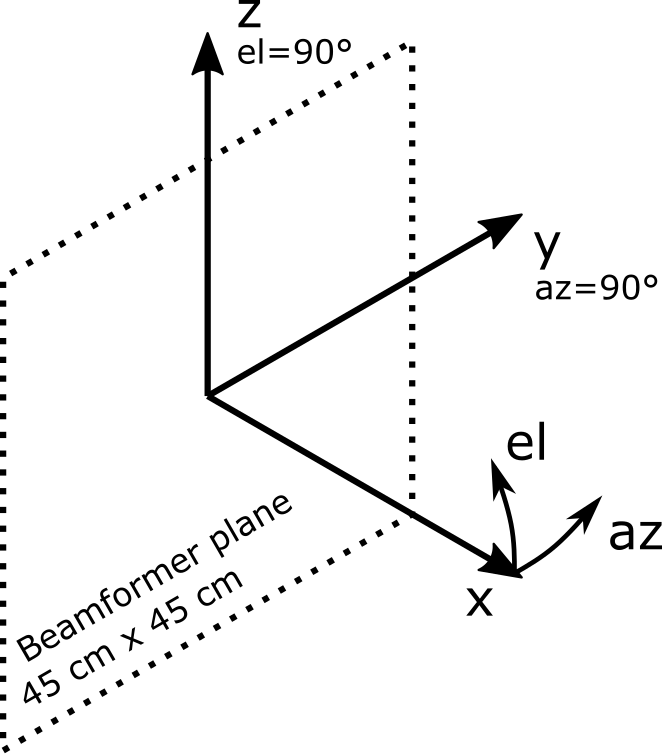
\includegraphics[width=0.4\textwidth]{coord.png}
	\caption{Reference coordinate system with available beamformer area}
	\label{fig:coord}
\end{figure}

Hydrophone operates in frequency range of 20 kHz to 90 kHz. The communication 
link uses a carrier frequency of 30 kHz. Hydrophone has a cosine radiation 
pattern, described by expression
\[ D(\phi,\theta) = \cos^2(\theta) \]
with $\phi$ being azimuth angle, and $\theta$ elevation angle. The radiation 
pattern is presented in the reference coordinate system in Figure 
\ref{fig:hydrophone}.
\begin{figure}[h!]
	\centering
	\subfigure[3D 
	view]{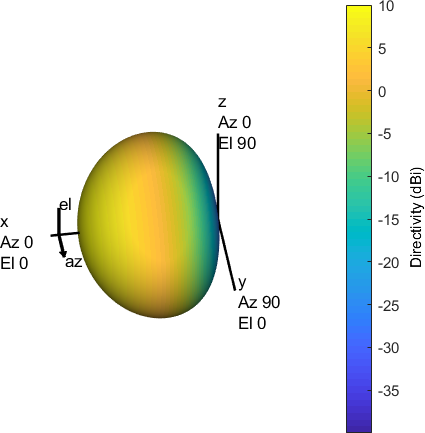
\includegraphics[width=0.415\textwidth]{hydrophone_3d.png}}
	\hfill
	\subfigure[Azimuth cut at 
	0deg]{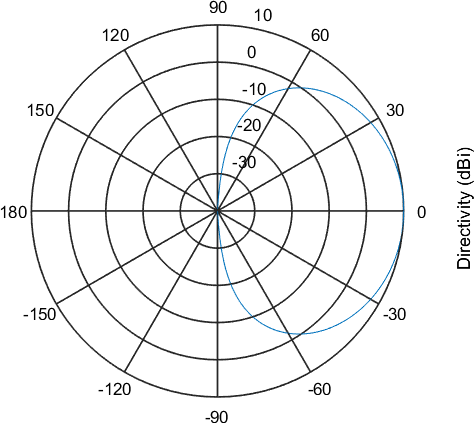
\includegraphics[width=0.45\textwidth]{hydrophone_cut.png}}
	\caption{Radiation pattern of a hydrophone element}
	\label{fig:hydrophone}
\end{figure}

Physically, hydrophones are circular, 5 cm in diameter. All hydrophones in the 
beamforming system are installed with their radiation maximum pointing to 
zenith, i.e. perpendicular to sea surface, as described in Figure 
\ref{fig:hydrophone}. At the other end, the ship is equipped with a single 
hydrophone mounted on ship's hull, and pointing at nadir, i.e. perpendicular to 
seabed.

Consider the signal narrowband. The ship is in the farfield of the beamforming 
system. Assume the communication link is being established in the Adriatic Sea, 
with average salinity of 38\textperthousand, and sea temperature of 20 
\textdegree C.

\subsection{Linear array}

Design a single linear antenna array along the y-axis to achieve the best link 
between the habitat and the ship in four given scenarios.
\begin{description}
	\item[Scenario 1] The ship is directly above the beamforming system.
	\item[Scenario 2] The ship is located along the longitudinal (y) axis of 
	the beamforming system, at an elevation of 30\textdegree.
	\item[Scenario 3] The ship is located along the longitudinal (y) axis of 
	the beamforming system, at an elevation of 60\textdegree.
	\item[Scenario 4] The ship is located along the longitudinal (y) axis of 
	the beamforming system, at an elevation of 70\textdegree.
\end{description}

\begin{figure}[h!]
	\centering
	\subfigure[Scenario 
	1]{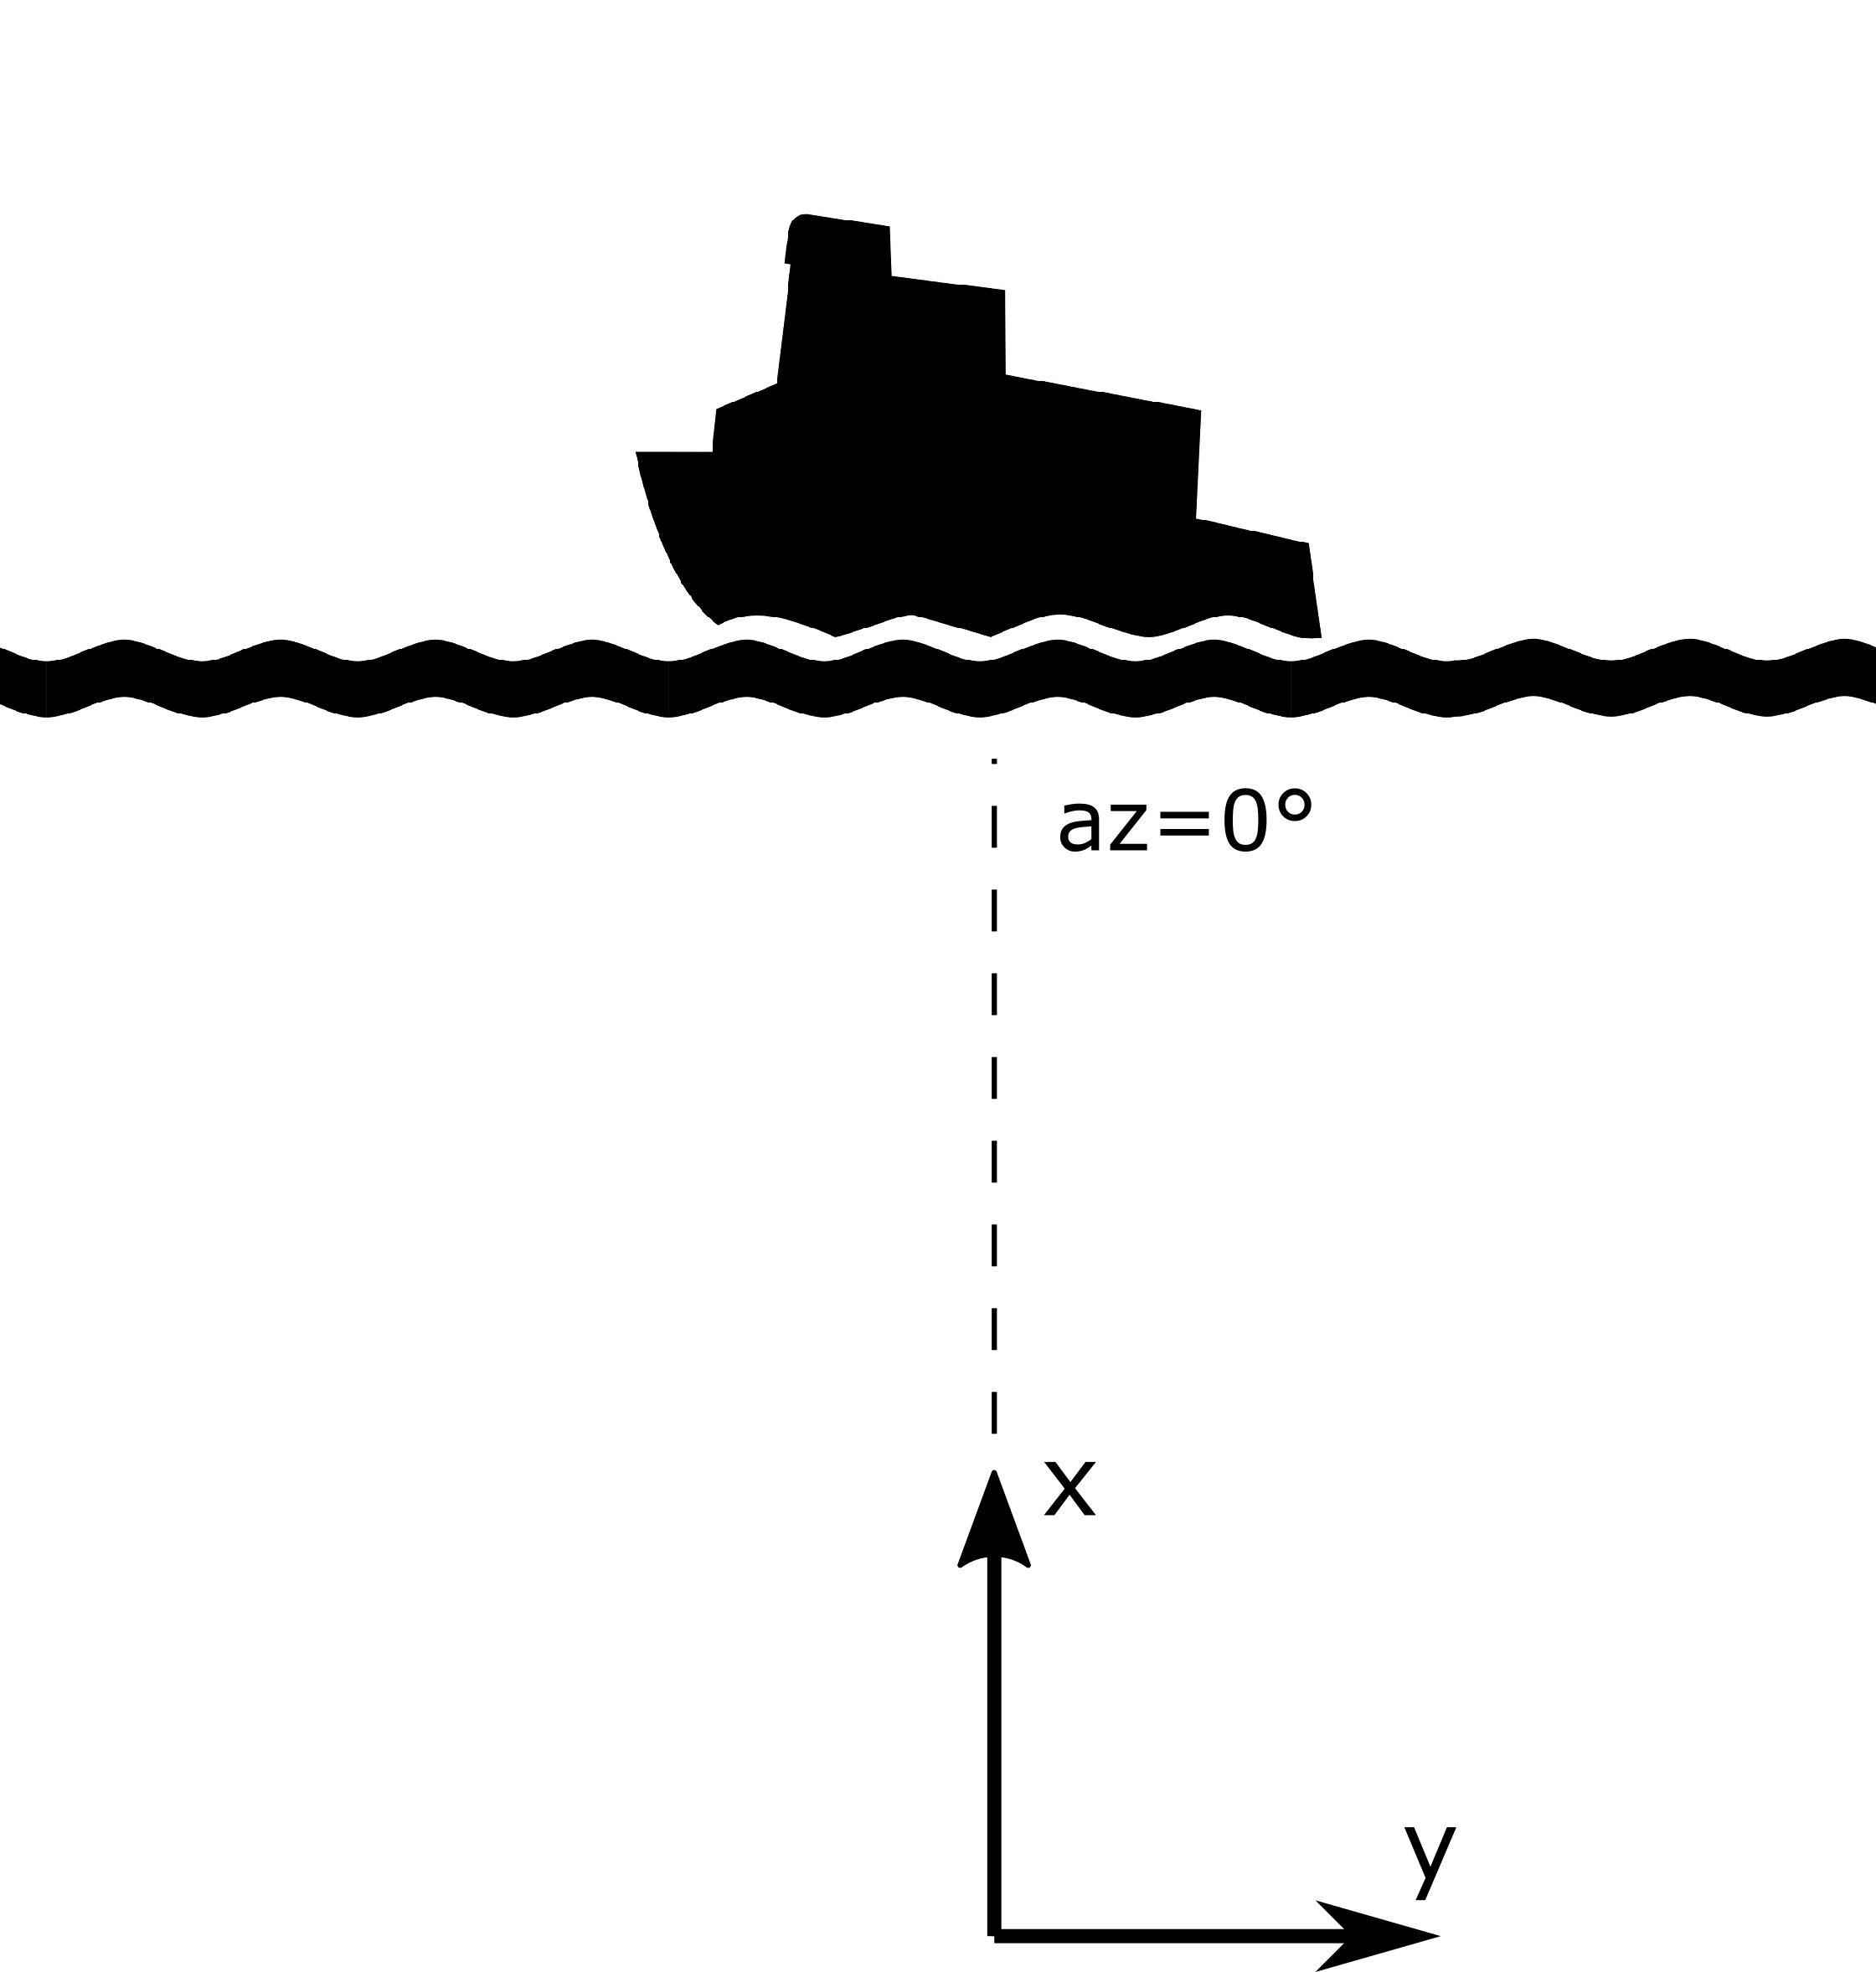
\includegraphics[width=0.45\textwidth]{scenario1.png}}
	\hfill
	\subfigure[Scenario 
	2]{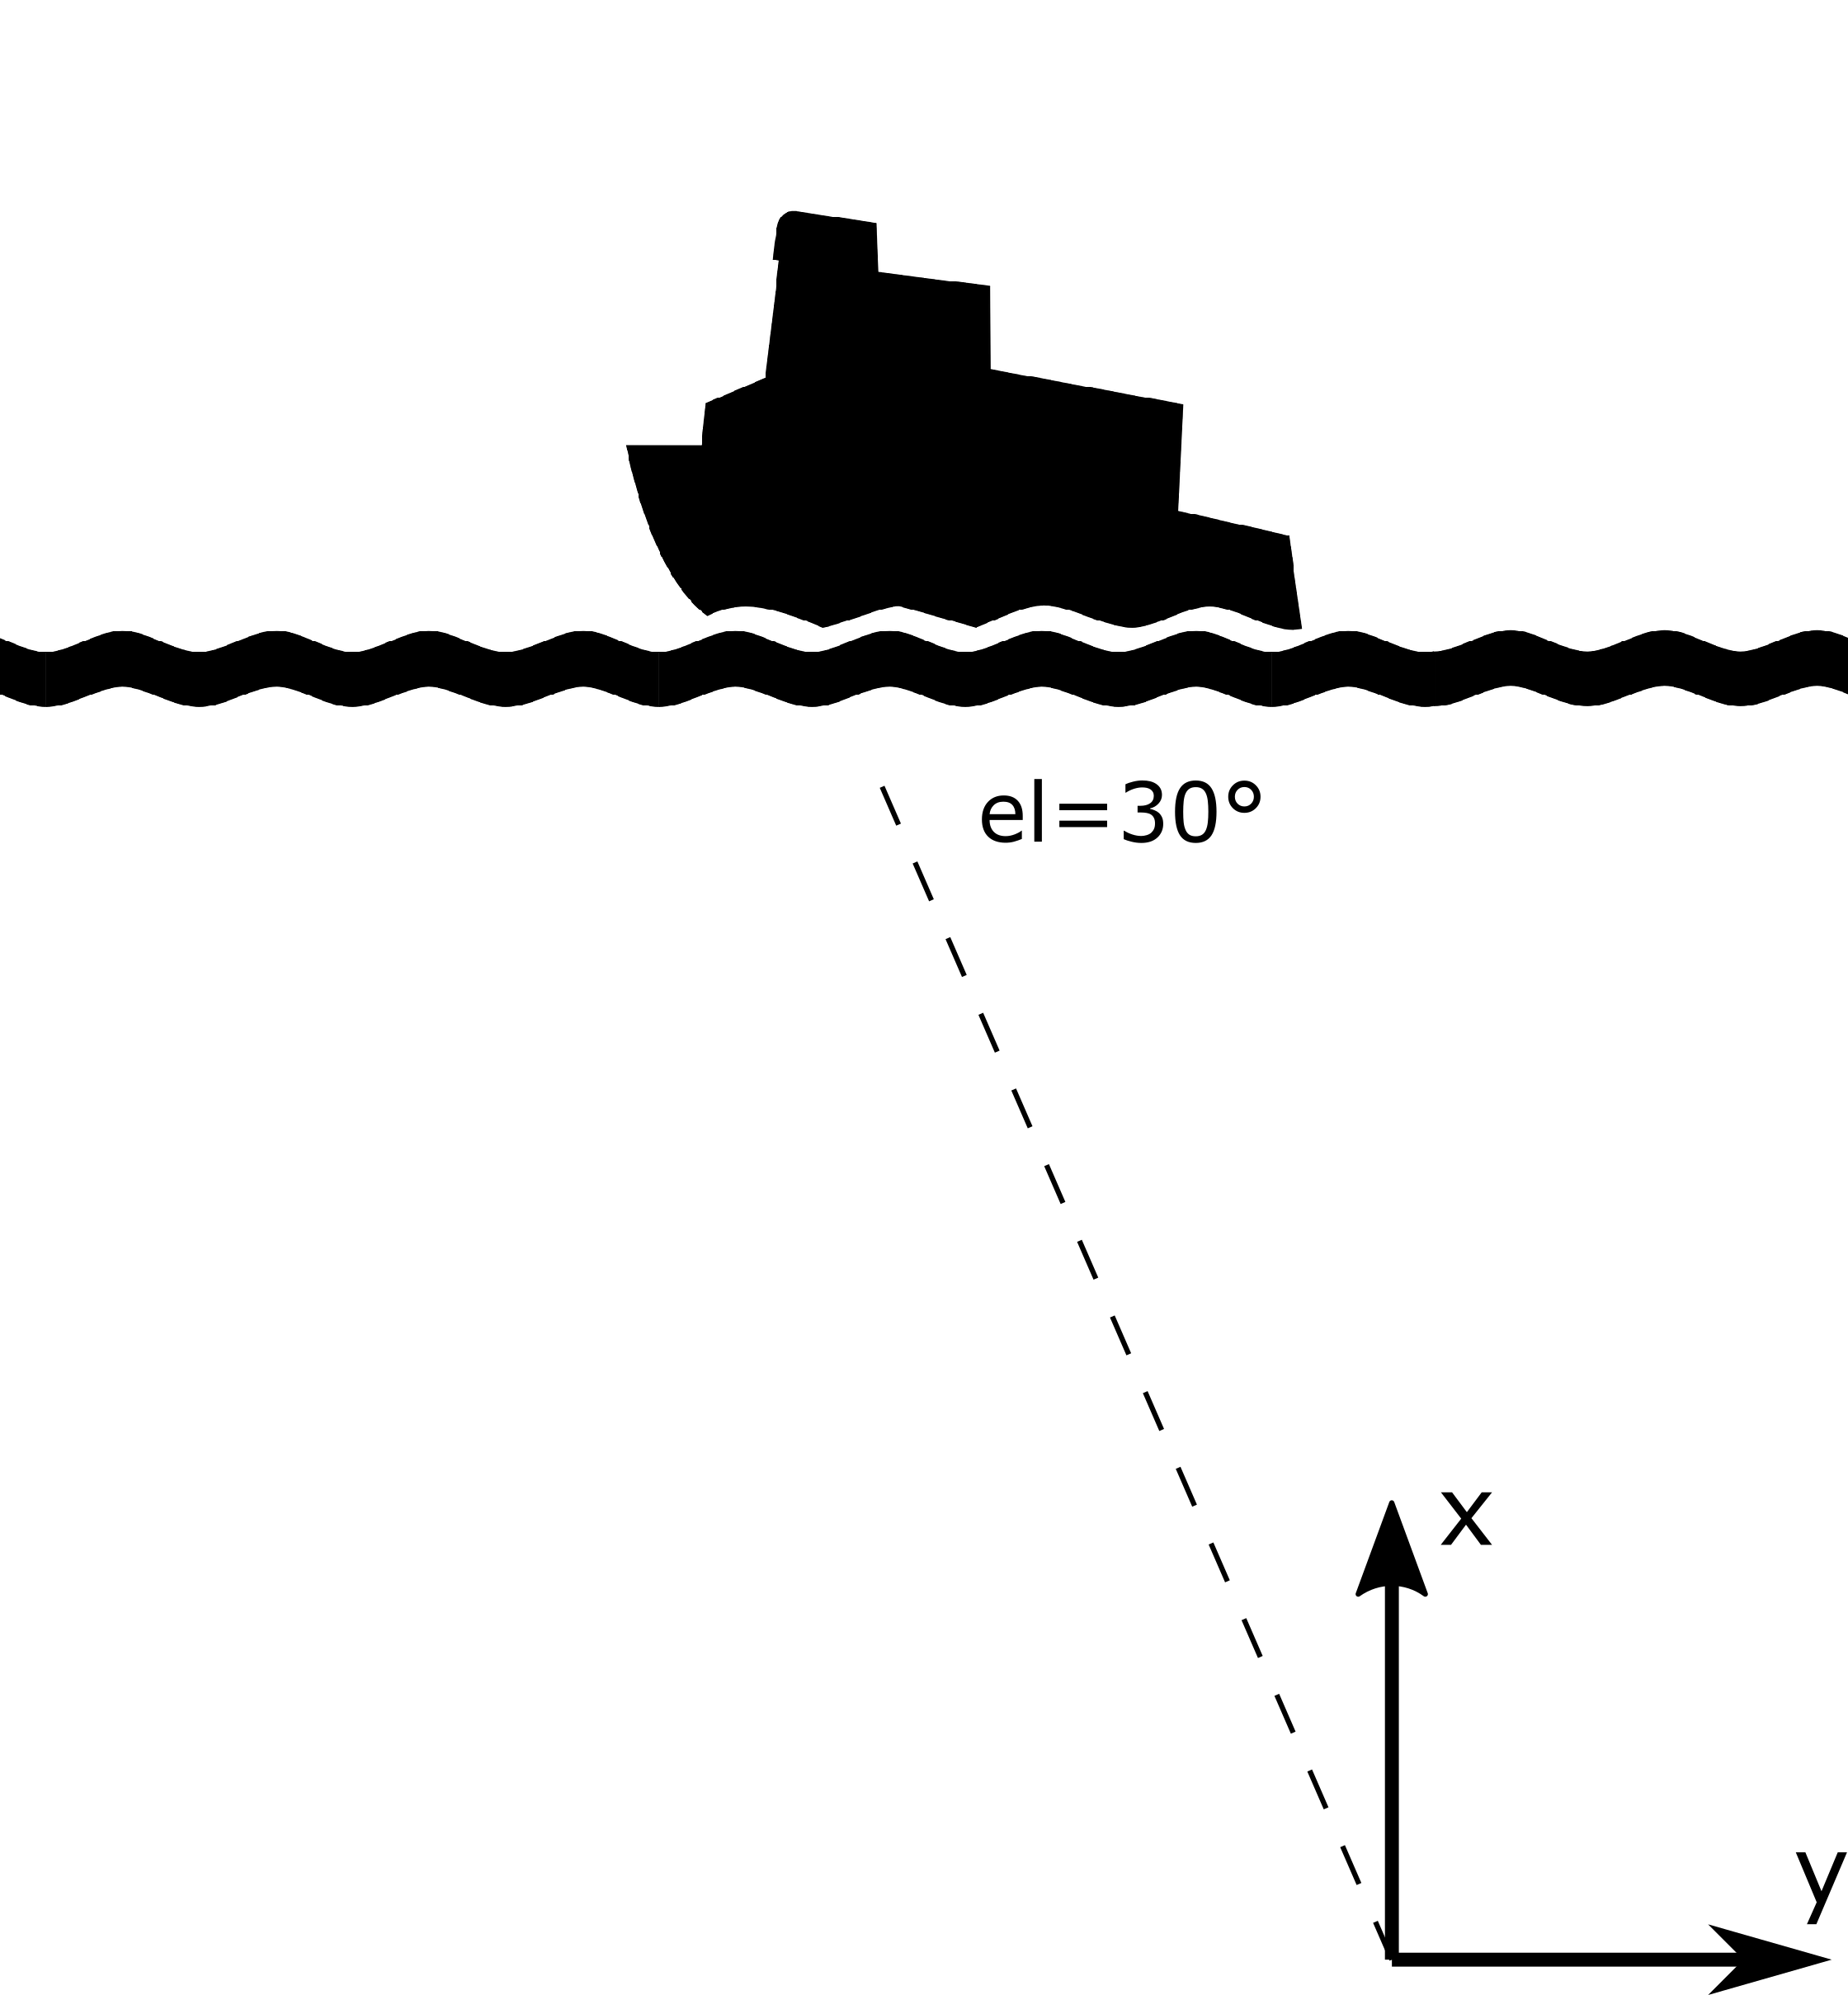
\includegraphics[width=0.45\textwidth]{scenario2.png}}
	\\
	\subfigure[Scenario 
	3]{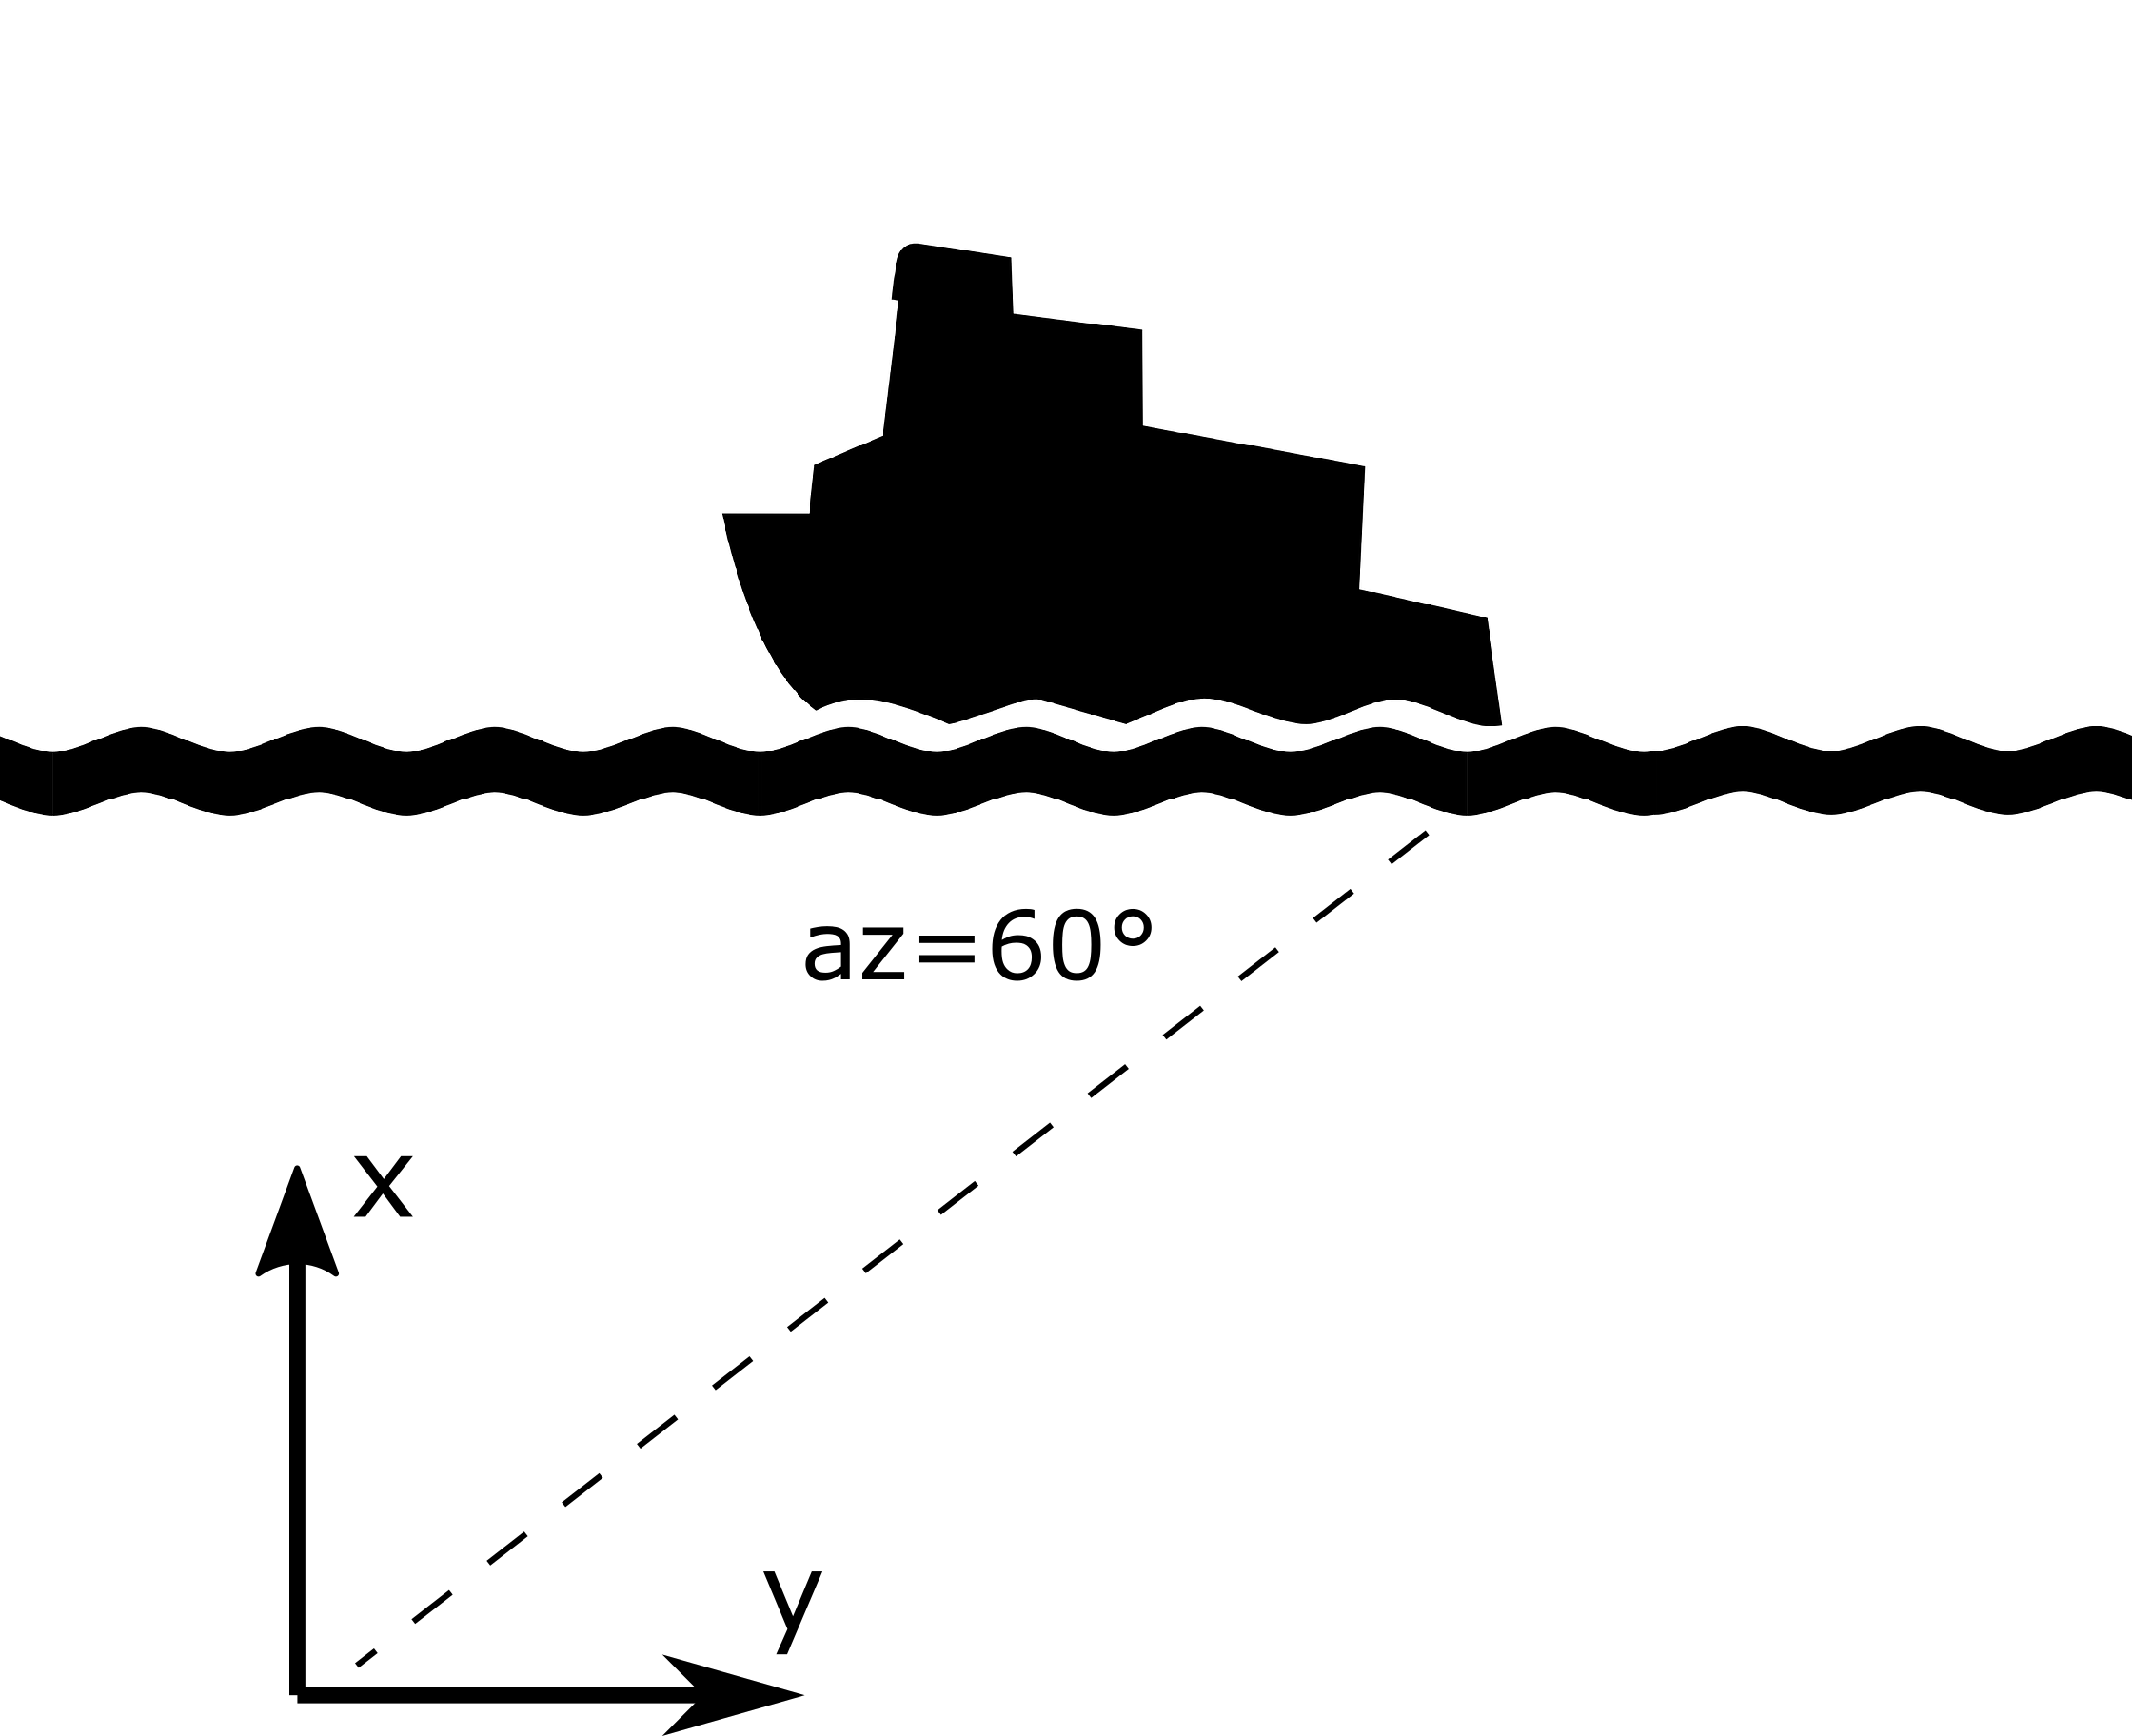
\includegraphics[width=0.45\textwidth]{scenario3.png}}
	\hfill
	\subfigure[Scenario 
	4]{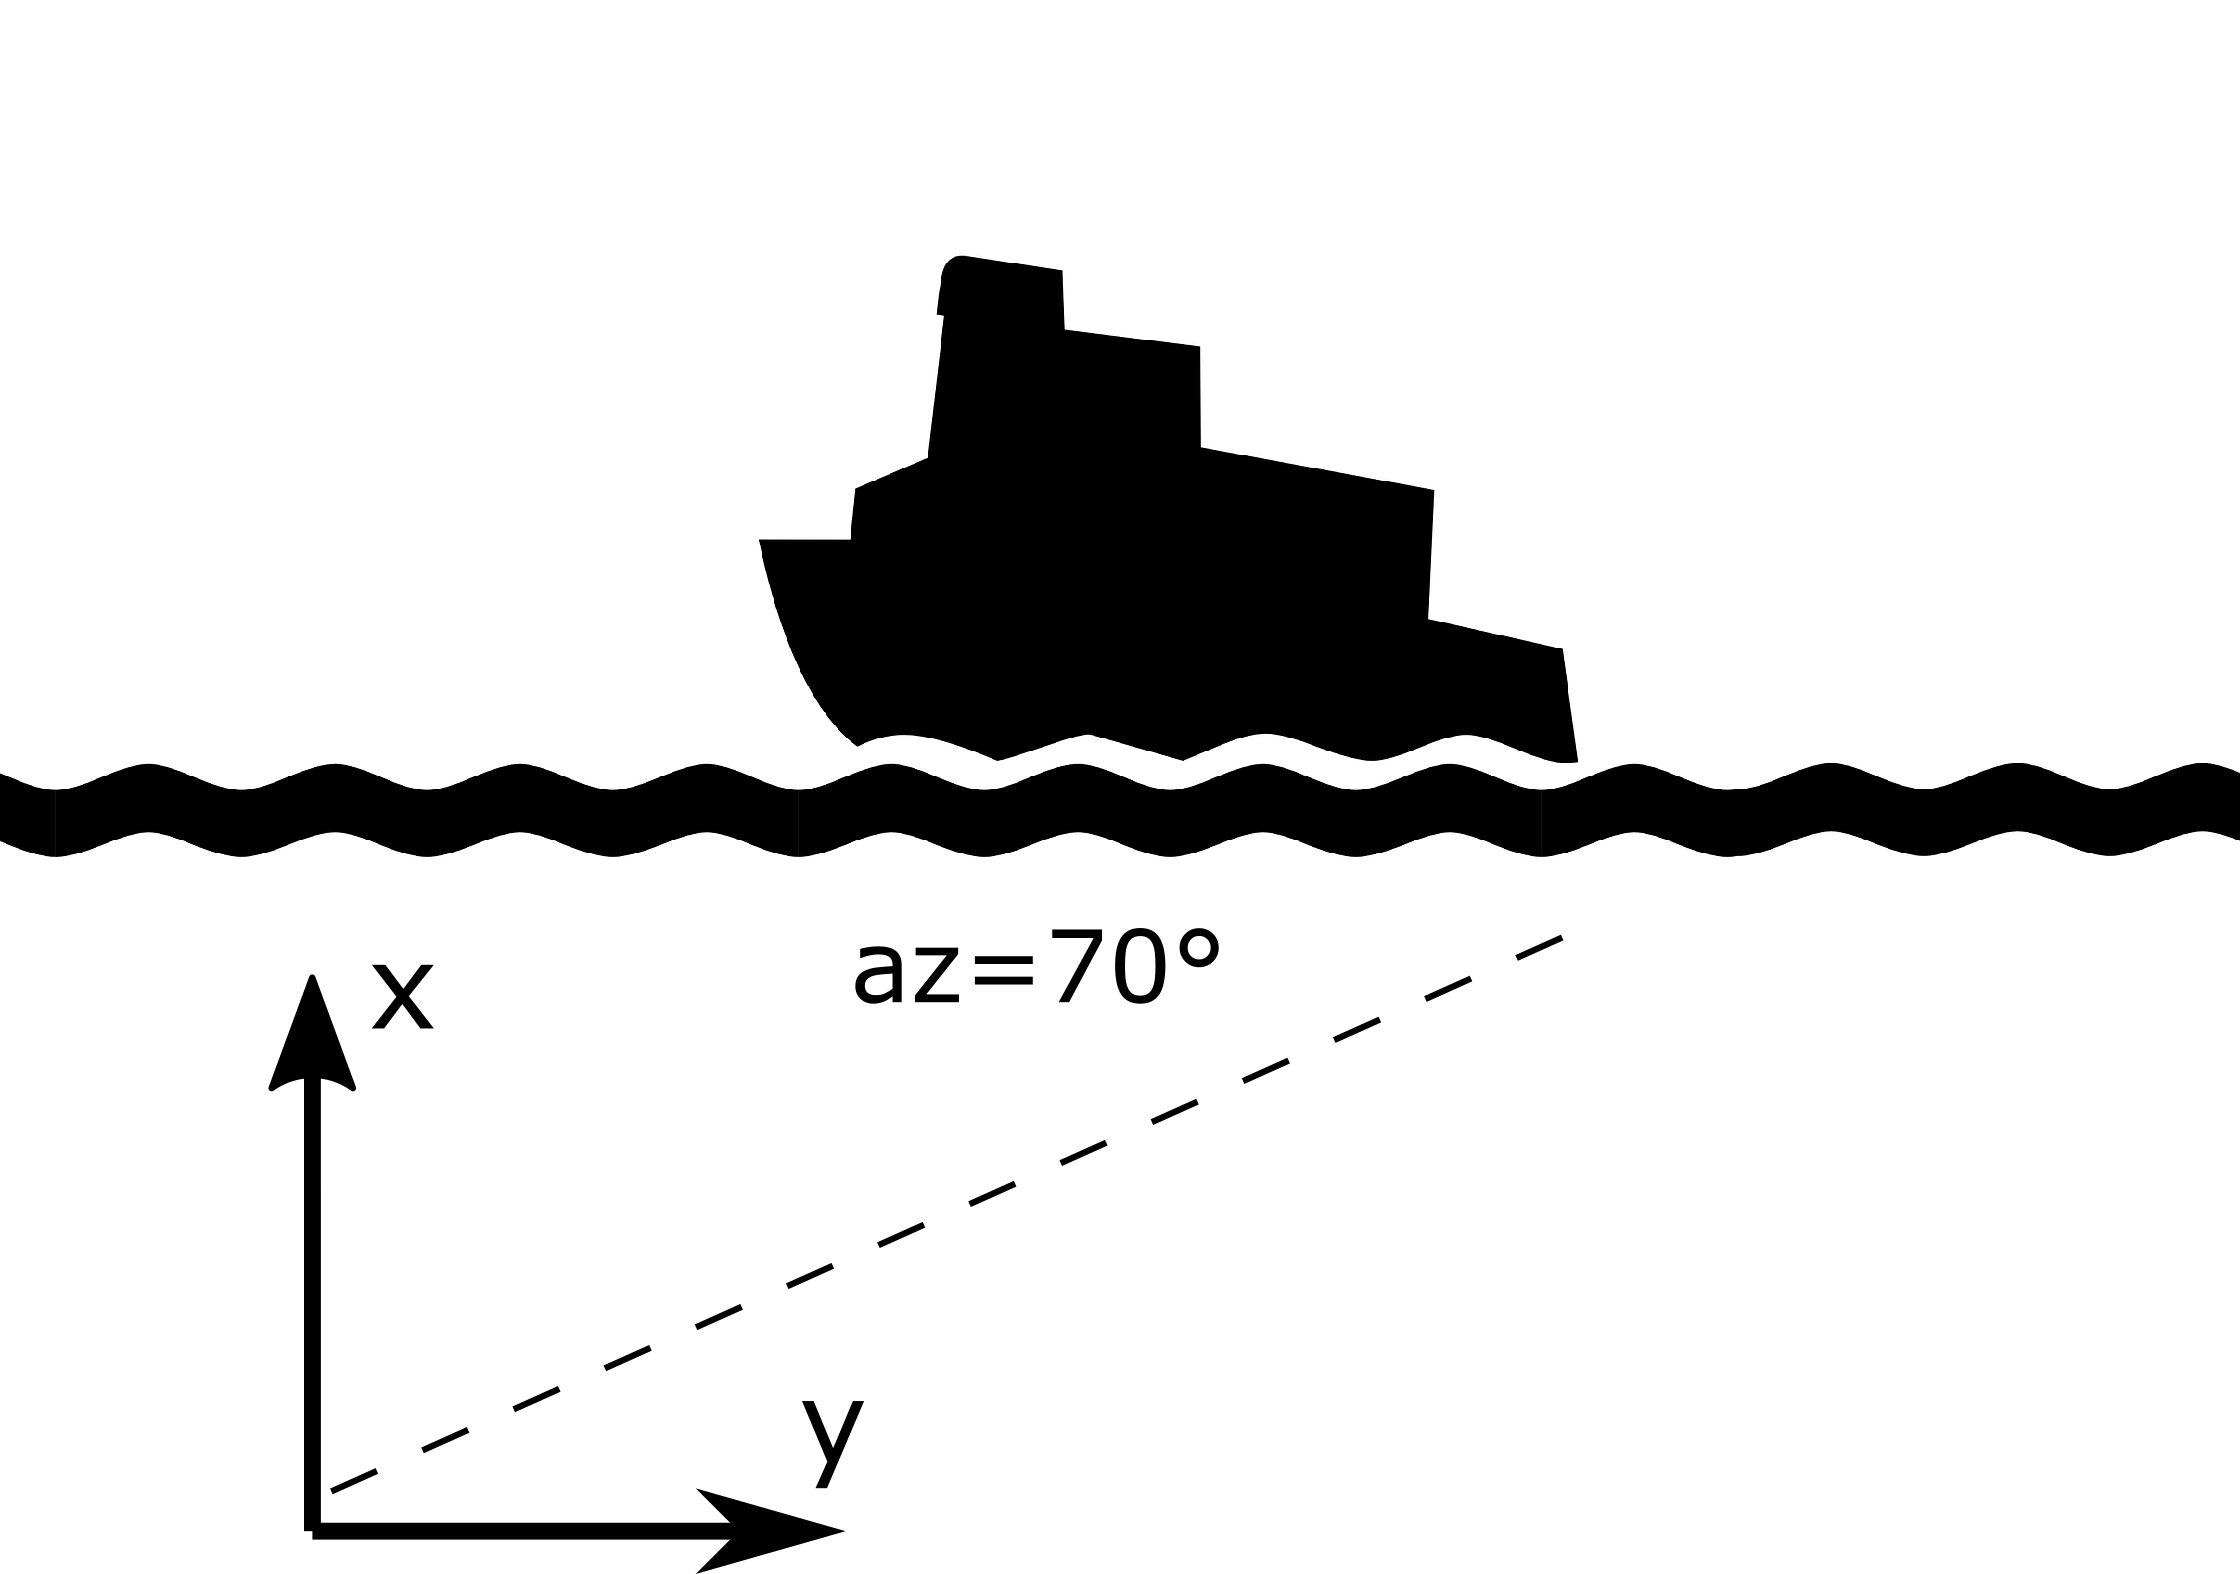
\includegraphics[width=0.45\textwidth]{scenario4.png}}
	\caption{Scenarios for Task 1}
\end{figure}

A beamforming system is defined by y coordinates of each hydrophone element. 
Number of elements is arbitrary, given the limitations introduced in 
Introduction. The same beamforming system is used for all four scenarios. For 
each of the four scenarios, provide complex weights that are applied to each of 
the hydrophone elements to achieve optimal beamforming for the particular 
scenario.

\subsubsection*{Output data}

\begin{description}
	\item[elements1.csv] \,\\ The file contains a one-dimensional array 
	representing the position of each hydrophone element along the y axis in 
	metres.
	
	\item[scenarioX.csv] \textit{e.g. scenario1.csv, \ldots}\,\\ The file 
	contains a one-dimensional array of complex numbers representing the 
	weights applied to each hydrophone element. Weights are given for elements 
	in the same order as they are listed in \textsf{elements1.csv}. Array 
	length is equal to the number of elements in the beamforming system. All 
	numbers are inside, or at the edge of the unit circle.
	
	Complex numbers should be stored either in
	\begin{itemize}
		\item cartesian notation: \textsf{a+bi}, or
		\item polar notation: \textsf{P*exp(Ri)}
	\end{itemize}
\end{description}


\subsubsection*{Scoring}

The beamforming system you designed is evaluated for each of the given 
scenarios. For the first three scenarios, points are awarded for the 
directivity the beamforming system achieves in the direction of the ship, after 
applying the given beamforming weights. If the ship is in the main lobe of the 
beamforming system, the number of awarded points is equal to
\[ D_\textrm{target} - \varDelta \phi \]
where $D_\textrm{target}$ is the directivity in the direction of the ship in 
dBi, and $\varDelta \phi$ the angular distance between the ship and the 
direction of beamformer's maximum directivity in degrees. If the ship is within 
the strongest sidelobe of the beamforming system, the number of awarded points 
is equal to
\[ D_\textrm{target} - \dfrac{\varDelta \phi}{10} \]
The ship is considered to be within a radiation lobe if it is within 6 dB of 
the considered radiation lobe's maximum radiation.

In scenario 4, the beamforming system is evaluated with the given beamforming 
weights, and its directivity compared to that of the same beamforming system 
with uniform excitation. The points are then awarded as
\[ D_\textrm{target,weighted} - D_\textrm{target,uniform} \]
The highest number of points for this scenario is 20.

For all scenarios, the following rules apply: A beamforming system constructed 
with just one element is awarded no points. A beamforming system acheiving 
negative directivity (in dBi) in the direction of the ship is awarded no points.

\subsection{Planar array}

You will now design a planar beamforming system, to enable beamforming toward a 
ship that is moving in both dimension along the sea surface. You are given a 
single scenario (\textit{Scenario 5}) in which the ship is located at an 
azimuth angle of 45\textdegree and at elevation of 60\textdegree, as seen from 
the reference coordinate system.

\subsubsection*{Output data}

\begin{description}
	\item[elements2.csv] \,\\ The file contains 2D coordinates of beamforming 
	elements. One row of the file represents one beamforming element. The first 
	column is the y-coordinate, and the second column is the z-coordinate.
	
	\item[scenario5.csv] \,\\ The file contains a one-dimensional array of 
	complex numbers representing the weights applied to each hydrophone 
	element. Weights are given for elements in the same order as they are 
	listed in \textsf{elements2.csv}. Array length is equal to the number of 
	elements in the beamforming system. All numbers are inside, or at the edge 
	of the unit circle.
	
	Complex numbers should be stored either in
	\begin{itemize}
		\item cartesian notation: \textsf{a+bi}, or
		\item polar notation: \textsf{P*exp(Ri)}
	\end{itemize}
\end{description}

\subsubsection*{Scoring}

The team will achieve points that correspond to directivity in dBi in the 
direction of the ship.

A beamforming system constructed with just one element is awarded no points. A 
beamforming system acheiving negative directivity (in dBi) in the direction of 
the ship is awarded no points.

\subsection{Evaluation and results}

Evaluations are performed automatically, and will run continuously during the 
competition day. You can see the results of evaluation for all teams on a 
scoring board, and thus monitor how everyone progresses. The scoring board can 
be found on \url{https://engineering.stemgames.hr}.

You submit your output files to your team's Google Drive folder.
After the simulation for your beamformer design is complete, you will find 
evaluator's log file on Google Drive.

The input files found on Google Drive at the end of the competition day will be 
taken as team's final solution. No changes will be accepted after that time.

At the end of the competition day, and after the final evaluations complete, 
the total number of points awarded to the team will be normalized to the best 
team. Hence, the best team will receive 10 points, and the points received by 
other teams will be linearly scaled to the best team.
		
\end{document}
